%!TEX root = ../thesis.tex
%*******************************************************************************
%*********************************** First Chapter *****************************
%*******************************************************************************

\chapter{Introduction}

\ifpdf
    \graphicspath{{Chapter1/Figs/Raster/}{Chapter1/Figs/PDF/}{Chapter1/Figs/}}
\else
    \graphicspath{{Chapter1/Figs/Vector/}{Chapter1/Figs/}}
\fi

\section{Assembly}
\subsection{DNA sequencing data types}
\par{
Before moving forward, it is important to understand the data types used. 
}

\subsubsection{Sanger sequencing}

\subsubsection{Short reads}


\subsubsection{PacBio}

\par{
Pacific Biosciences (PacBio) uses microscopic wells known as zero-mode waveguides (ZMWs) along with single molecules of DNA and DNA polymerase to optically measure fluorescent nucleotides as they are incorporated by the polymerase. This is known as single molecule real-time sequencing (SMRT sequencing). The DNA template is prepared with hairpin adapter sequences known as the SMRTbell adapters. This allows for multiple passes of the same DNA molecule. Initially, polymerase nucleotide incorporation and optical measurement speed were limited. That combined with the rate at which molecules dissociate from the ZMW limited the number of times long molecules could be sequenced to once or just a few times. This results in long, but noisy reads with roughly 15\% error rate\cite{pacbio}\cite{blasr}\cite{clrerror} known as continuous long reads (CLR). The PacBio data used in Chapter 3 is CLR data. More recently, advances in the speed of polymerase nucleotide incorporation and optical measurements have allowed for many passes of the same long molecules. This allows for circular consensus sequencing (CCS aka HIgh FIdelity sequencing or HIFI) across these multiple passes and much higher accuracy (<1\% error rate on average) while maintaining true single molecule sequencing\cite{HIFI}. The PacBio data used in Chapter 4 is CCS data.
}


\begin{figure}[htbp!]

\caption{Circular consensus sequencing}
\label{figure:ccs}
\begin{centering}
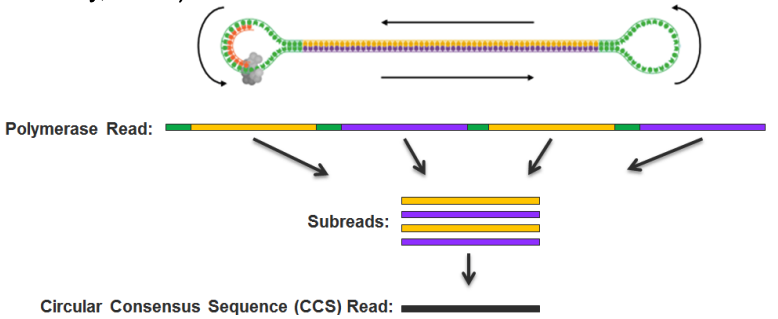
\includegraphics[width=0.65\textwidth]{CCS.png}
\par{Diagram outlining circular consensus sequencing (credit: PacBio website).}
\end{centering}
\end{figure}

\subsubsection{Linked reads}

\par{
The 10X platform starts with high molecular weight DNA input into a microfluidic system that partitions those long DNA molecules into ?GEMs? (Gel bead in EMulsion) with oil surrounding an aqueous solution containing the DNA and reagents with a gel bead housing millions of copies of an oligo containing random primers, Illumina adapters, and the same barcode DNA sequence. Each different gel bead has a different barcode DNA sequence with high probability. Each GEM is poisson loaded with HMW DNA and on average gets roughly ten long molecules in the standard workflow. Short sequences are then amplified from these long molecules with random priming which creates a construct with the Illumina P5 and P7 adapters, the barcode oligo, and the DNA insert. This is then sequenced using standard short read Illumina sequencing. All of the reads with the same barcode sequence come from the same GEM and thus from a handful of long molecules. When the reads are mapped to a reference genome, the reads from each barcode cluster into a few small regions of the genome associated with their molecule of origin. This long range information can then be used to map into repeat regions of the genome, phase haplotypes, and call structural variation \cite{10xlinked}.
}

\begin{figure}[htbp!]

\caption{10x Genomics Linked reads}
\label{figure:linkedreads}
\begin{centering}
\sidesubfloat[]{
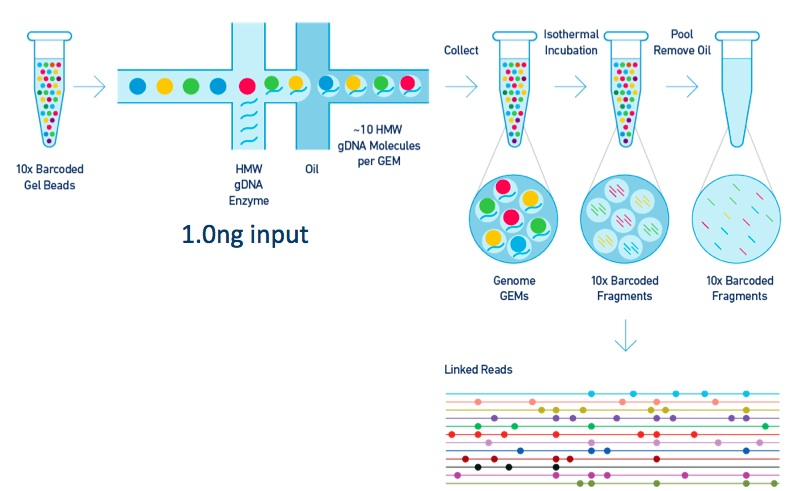
\includegraphics[width=0.65\textwidth]{linkedreads.jpeg} \label{fig:a}
} \\
\sidesubfloat[]{
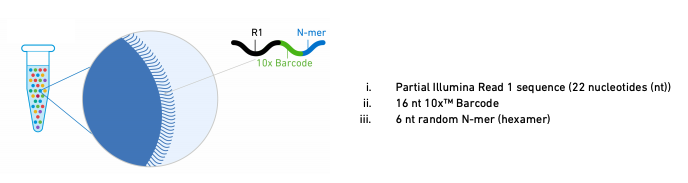
\includegraphics[width=0.65\textwidth]{gem.png} \label{fig:b}
} \\
\sidesubfloat[]{
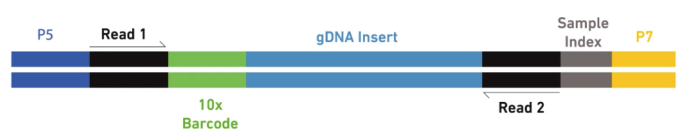
\includegraphics[width=0.65\textwidth]{construct.png} \label{fig:c}
}
\par{\textbf{a)} outlines the microfluidic system to create the Gel bead in reverse emulsion. \textbf{b)} shows the gel bead oligo setup and \textbf{c)} diagrams the final construct. (image credits to 10xgenomics website)}
\end{centering}
\end{figure}

\par{
While 10x Genomics Linked reads are used in Chapter 4, the technology is no longer offered by that company. More recently, bead based systems have been developed that do not require a microfluidic system. In solution with microbeads, long DNA molecules tend to wrap around a single bead\cite{beadphasing}\cite{LFR}. Separately, Tn5 transposase has been used to insert adapter and barcode sequences at high frequency into genomic DNA\cite{cptseq}. With these ideas combined, Frank Chan's group has developed a technique called Haplotagging which uses microbeads bound to Tn5 transposase with one of 85 million molecular barcodes and Illumina sequencing adapters creating linked read libraries for a fraction of the price in a single tube\cite{haplotagging}.
}

\subsubsection{High throughput chromatin conformation capture (Hi-C)}



\subsection{Reference Genomes}
\subsubsection{Resequencing}
\subsubsection{Read Mapping}
\subsubsection{Variant Calling}
\subsubsection{Population Genomics}

\subsubsection{The old way}
\subsubsection{The new way and Darwin Tree of Life and Earth Biogenome Project}

\subsection{Haplotype phasing}
\subsubsection{Statistical}
\subsubsection{Direct / Read based}

\subsection{Assembly}
\subsubsection{Overlap, Layout, Consensus}
\subsubsection{De brujin graphs}
\subsubsection{String graphs}
\subsubsection{Repeats, Heterozygosity, and Errors}
\subsubsection{Trio binning}
\subsubsection{Haploid assembly: Hytaditiform moles, seeds}
\subsubsection{Phased assembly}


\subsection{Post assembly manipulations}
\subsubsection{Polishing}
\subsubsection{Haplotig purging}
\subsubsection{Scaffolding}

\subsection{Assembly validation}
\subsubsection{Kmer based methods}
\subsubsection{Gene based methods}
\subsubsection{Contamination detection}

\section{Single Cell}
\subsection{Background and Motivation}
\subsection{Technologies}
\subsubsection{Single cell RNA sequencing}
\subsubsection{Single nucleus RNA sequencing}
\subsubsection{Single cell ATAC sequencing}
\subsubsection{Single cell DNA sequencing}

\subsection{Analysis of scRNAseq data}
\subsubsection{Barcode correction}
\subsubsection{Cell-barcode detection}
\subsubsection{Visualization}
\subsubsection{Cell type clustering and annotation}
\subsubsection{Doublet detection}
\subsubsection{Ambient RNA detection}
\subsection{Downstream analysis}
\subsubsection{Trajectories}
\subsubsection{Pseudotime}
\subsubsection{RNA velocity}
\subsubsection{Differential Isoforms}
\subsubsection{Genetic Variation}




\subsection{Batch effects}
\subsection{Ambient RNA}

\subsection{Mixtures}
